\documentclass[10pt]{article}
\usepackage[a4paper,left=15mm,right=15mm,top=16mm,bottom=16mm]{geometry}
\usepackage{fontspec,graphicx,xcolor}
\setmainfont{Arial}
\setsansfont{Arial}
\pagestyle{empty}
\setlength{\parindent}{0pt}
\setlength{\parskip}{0pt}
\setlength{\emergencystretch}{1em}
\begin{document}
{\fontsize{13}{16}\selectfont\bfseries Figure 1}\par\vspace{3mm}
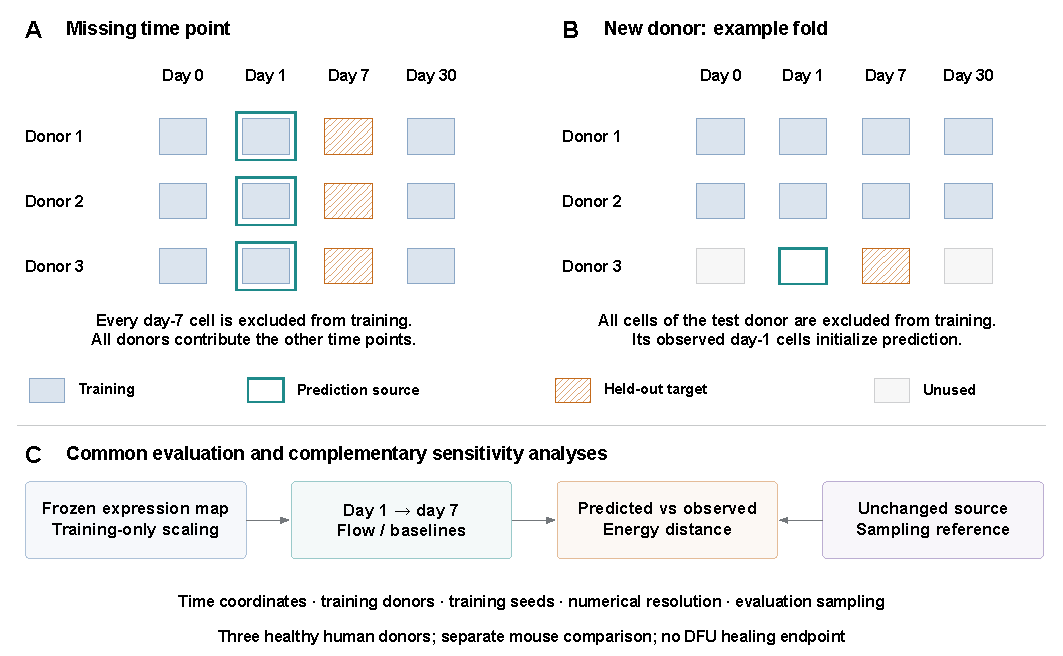
\includegraphics[width=180mm]{../figure1_workflow.pdf}\par\vspace{3mm}
{\fontsize{9}{11.5}\selectfont Acute-wound sampling and frozen-coordinate flow. (A) Conceptual repair, not measured histology or closure time, and repeated biopsies of three healthy donors at days 0, 1, 7 and 30. The lower route starts with 7,002-gene proportions: 5,383 panel genes are covered and the remainder zero-filled. A frozen 15-dimensional encoder mean μ is scaled using training cells only. A shared conditional-flow-matching (CFM) field learns from independently sampled product-coupled endpoints; 50-step RK4 predicts the day-7 marginal in scaled μ coordinates, not simplex weights. All day-7 cells are held from fitting and scaling. This is global time holdout, not the separate held-donor task that permits training-donor day-7 cells. (B) A uniform 2,000-cell display subset of 12,259 fibroblasts by time. PCA and scaling exclude day 7; the axes explain 43.5\% and 10.6\% of training variance. (C) The same cells by donor. (D) Twelve measured genes per donor--time biopsy, with log-transformed pseudobulk counts per 10,000 scaled separately by gene; colors do not compare absolute levels between genes. (E) Fibroblast counts per biopsy; cells are not independent donors. (F) Thirty-six seed-0 numerical paths from observed day-1 cells to day-7 rank time over the day-1/day-7 display. Arrows are not tracked cell fates; errors use all 15 coordinates.\par}
\newpage
{\fontsize{13}{16}\selectfont\bfseries Figure 2}\par\vspace{3mm}
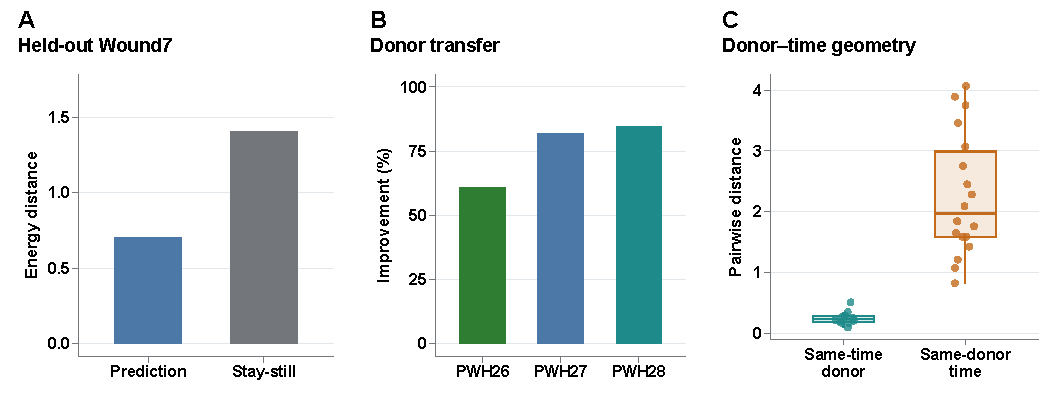
\includegraphics[width=180mm]{../figure2_wound7_transfer.pdf}\par\vspace{3mm}
{\fontsize{9}{11.5}\selectfont Global Wound7 reconstruction, donor transfer and donor--time geometry. (A) Bars show predicted and stay-still energy distances to pooled Wound7 after excluding that time globally; relative improvement is 100 times (stay-still minus predicted distance) divided by stay-still distance, giving 49.9\%. (B) Each bar is a genuinely held-out donor, with all four times retained in the other two donors; the mean relative improvement is 75.9\%. Bars are point estimates without confidence intervals. (C) Points show 12 between-donor same-time distances and 18 within-donor between-time distances. Boxes span the interquartile range, centre lines are medians, and whiskers extend to extreme points within 1.5 interquartile ranges. The temporal/donor median ratio is 8.46 (10,000-draw descriptive pair-distance resampling range, 2.5th--97.5th percentiles, 6.02--13.11). All distances use training-standardized latent coordinates. Shared donors make these pairs dependent; the range has no established donor-population coverage. Three healthy donors do not provide DFU prediction validation.\par}
\newpage
{\fontsize{13}{16}\selectfont\bfseries Figure 3}\par\vspace{3mm}
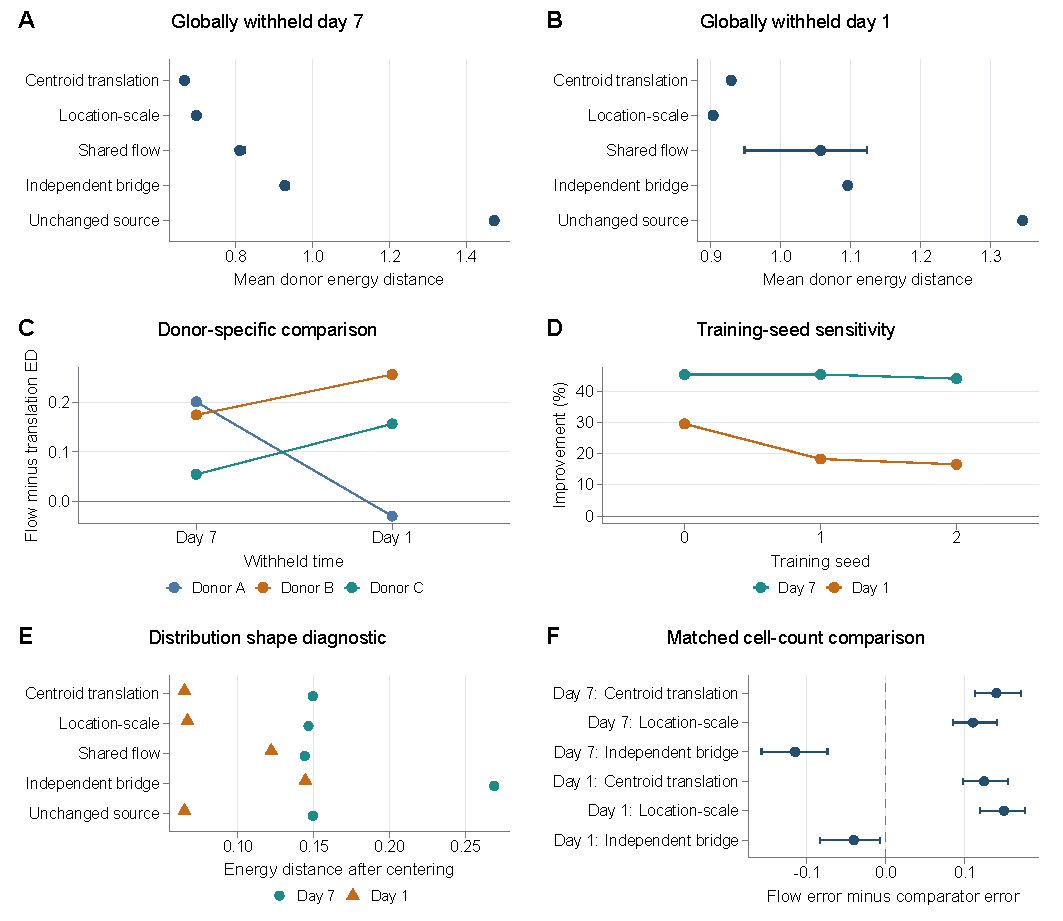
\includegraphics[width=180mm]{../figure3_interpolation_controls.pdf}\par\vspace{3mm}
{\fontsize{9}{11.5}\selectfont Simple baselines for globally missing times. All methods use the same frozen representation and training exclusions; error averages full-cell empirical energy distances within the three donors. (A) Withheld day 7, predicted from day 1 with day 30 as the observed anchor. (B) Withheld day 1, predicted from intact skin with day 7 as anchor. Points show the three-seed mean error; horizontal ranges show seed minima and maxima, not confidence intervals. Both tasks use the fixed rank-time interpolation fraction one half. (C) Donor-specific seed-averaged field error minus centroid-translation error; positive values favor translation. The later anchor belongs to the same donor, so this is retrospective interpolation rather than source-only donor transfer. (D) Each field seed's improvement over the corresponding unchanged source. Seeds and repeated distance evaluations provide no additional biological replication. (E) Seed- and donor-averaged energy distance after separately centering each distribution; this diagnoses shape without decomposing total error. (F) Mean and full range of flow-minus-comparator errors across 50 paired draws of 200 source and 200 target cells per donor; positive values favor the comparator. Location--scale uses only endpoint means and coordinate standard deviations. Matched draw ranges are not confidence intervals.\par}
\newpage
{\fontsize{13}{16}\selectfont\bfseries Figure 4}\par\vspace{3mm}
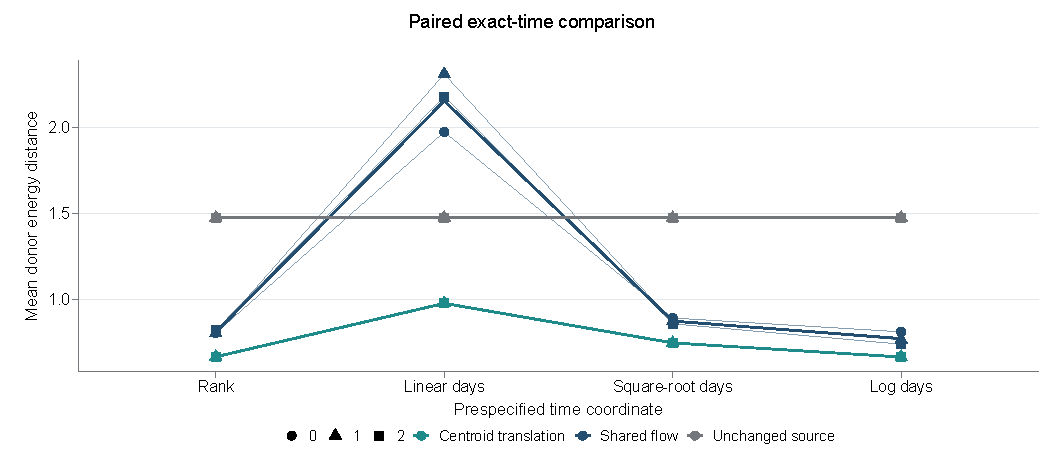
\includegraphics[width=180mm]{../figure4_time_axes.pdf}\par\vspace{3mm}
{\fontsize{9}{11.5}\selectfont Paired time-coordinate sensitivity under global day-7 holdout in three healthy donors. Twelve fields combine four fixed clocks with seeds 0, 1 and 2, each using 8,000 training steps and batch size 256. Network initialization, endpoint draws and interpolation random draws are paired across clocks within seed. All day-7 cells are excluded from fitting and scaling. Energy distance is evaluated at the exact transformed day-7 time after 50 RK4 steps, using the same source and target rows across clocks and seeds and a 1,200-cell cap per donor. Each point is the equal mean of three donor-specific distances; shapes identify training seeds. Thin lines join the same seed, and thick lines show three-seed means. Colors distinguish shared flow, within-donor centroid translation and unchanged source. The centroid control uses the permitted day-1 and day-30 biopsies, not day-7 expression. Constant baseline points overlap. Connecting categorical clock choices does not depict a biological trajectory, and seed spread is not a biological confidence interval.\par}
\newpage
{\fontsize{13}{16}\selectfont\bfseries Figure 5}\par\vspace{3mm}
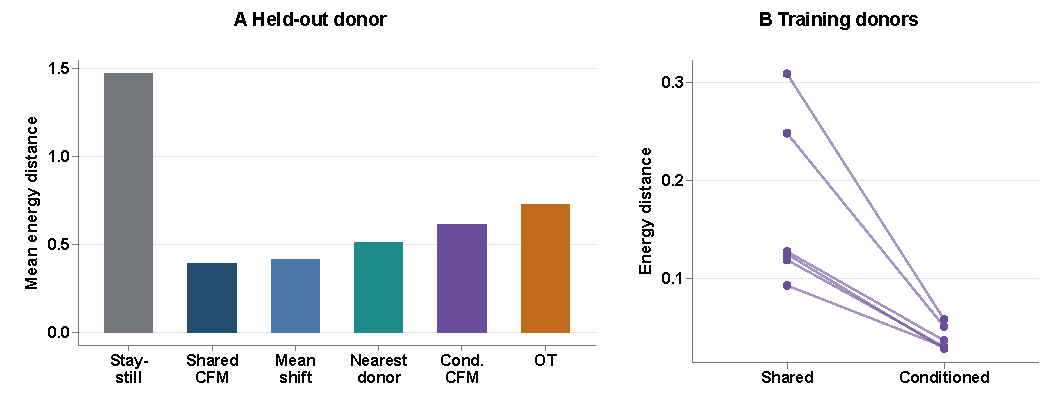
\includegraphics[width=180mm]{../figure5_methods_benchmark.pdf}\par\vspace{3mm}
{\fontsize{9}{11.5}\selectfont Method comparison across three held-out donors. (A) Bars are equally donor-weighted mean energy distances for unchanged source, five historical predictors and the added matched-particle target marginal. CFM means conditional flow matching; OT is the entropic transport displacement extension. The target marginal assigns equal mass to the two training donors' Wound7 distributions, uses no held-source expression, and averages 50 draws under the original target samples and scaling. Its mean error is 0.1818 versus 0.3947 for historical shared CFM, but PWH28 favors the field. All historical predictive methods exceed the single split-half gain reference in 3/3 folds; this descriptive criterion is not a significance test or population ranking. (B) Lines connect shared and conditioned errors for six training-donor comparisons (two retained donors in each of three fits). Conditioning improves all six. These comparisons share donors and do not measure unseen-donor transfer. Neither panel shows uncertainty intervals.\par}
\newpage
{\fontsize{13}{16}\selectfont\bfseries Figure 6}\par\vspace{3mm}
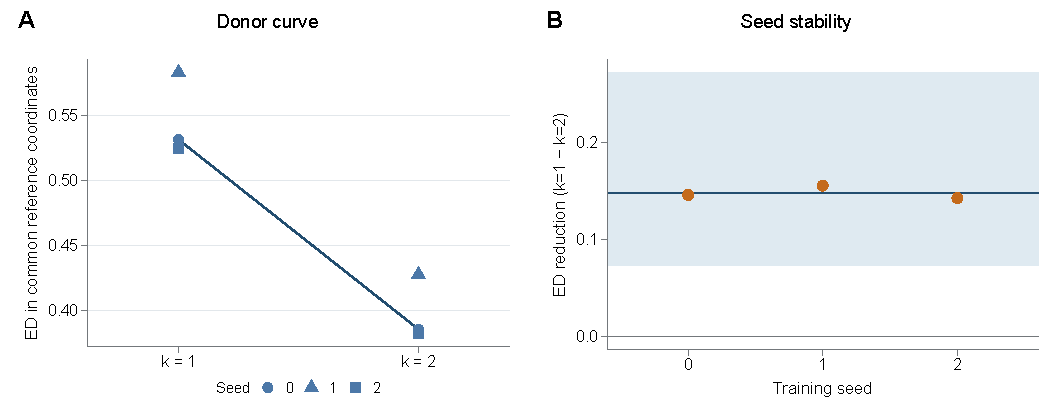
\includegraphics[width=180mm]{../figure6_donor_curve_stability.pdf}\par\vspace{3mm}
{\fontsize{9}{11.5}\selectfont Donor-count comparison in common scoring coordinates. (A) k is the number of training donors. The line joins seed-0 mean held-out errors, 0.5315 at k=1 and 0.3854 at k=2; symbols identify seeds 0, 1 and 2. Each model uses only its selected training donors for fitting and normalization. Predictions return to encoder coordinates before scoring under one reference fitted from both non-held donors, fixed across k and seed and excluded from single-donor fitting. At k=1, two training choices are averaged within held donor before equally weighting the three donors. (B) Points are seed-specific reductions, k=1 minus k=2. The line is the three-seed mean, 0.1483. Shading is a descriptive percentile 95\% range [0.0732, 0.2727] from 4,000 resamples of three donor blocks after seed averaging; it is not an interval for each point. Source and target indices are fixed. The largest configuration-specific seed range is 0.3377. Overlapping training sets limit interval interpretation, and two k values cannot identify a plateau or required cohort size.\par}
\newpage
{\fontsize{13}{16}\selectfont\bfseries Figure 7}\par\vspace{3mm}
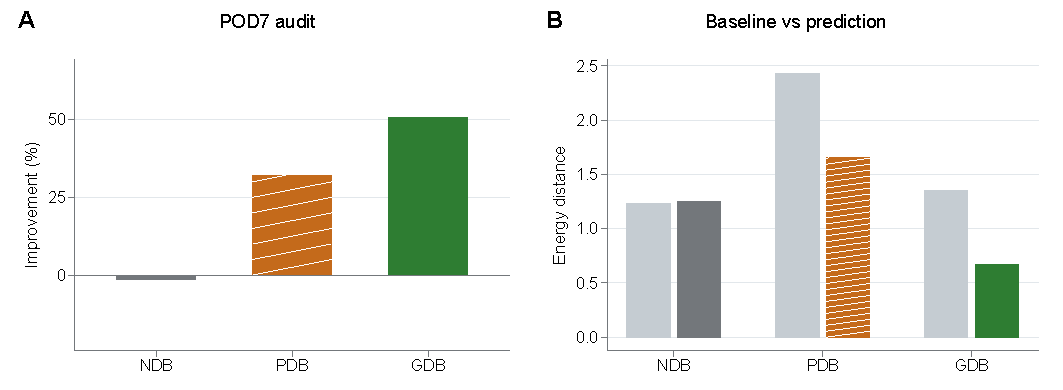
\includegraphics[width=180mm]{../figure7_mouse_arms.pdf}\par\vspace{3mm}
{\fontsize{9}{11.5}\selectfont Mouse POD7 computational audit for the source-labelled NDB, PDB and GDB arms. POD7 is excluded from fitting and scaling; rank-time fields trained at POD0, POD2 and POD30 predict from the observed POD2 source. (A) Relative energy-distance improvements over stay-still are −1.5\%, +32.1\% and +50.6\%. Hatching marks PDB, whose POD7 target fails the endpoint-distance ordering diagnostic. (B) Within each arm, the left grey bar is stay-still and the right coloured bar is prediction; hatching carries the same diagnostic meaning. The screen compares endpoint distances and does not prove or disprove geodesic interpolation. Each arm has one animal per time point and 4,182/7,002 mapped panel genes. Bars have no uncertainty intervals; cell counts do not supply independent animal replication or cross-species clinical validation.\par}
\end{document}
